\documentclass[11pt]{article}

\usepackage[letterpaper, margin=1in]{geometry}
\usepackage{amsmath, amssymb}
\usepackage{siunitx}
\usepackage{microtype}
\usepackage[hidelinks, colorlinks=true, urlcolor=blue!50!black]{hyperref}
\usepackage{xcolor}
\usepackage{booktabs}
\usepackage{enumitem}
\usepackage{tikz}
\usetikzlibrary{calc, decorations.pathreplacing, arrows.meta}
\usepackage{newtxtext, newtxmath}

\setlist{itemsep=2pt, topsep=4pt}

\newcommand{\dwdT}{\mathrm{d}W/\mathrm{d}T}
% \degC removed 2026-07-02; use siunitx \unit{\celsius} or \qty{...}{\celsius} instead.
\newcommand{\code}[1]{\texttt{#1}}

\title{TG-Analysis: a guided tour of the methods}
\author{Companion document to the \code{tga-analyze} script}
\date{}

\begin{document}
\maketitle

\noindent
This is a tutorial-style walk through the numerical methods behind the
\code{tga-analyze} script. It assumes you know what a TGA trace is and
how to read one but does not assume any background in signal processing,
nonlinear least squares, or thermal-analysis kinetics. The goal is for
the methods to feel obvious by the end, not opaque.

\tableofcontents

\section{What the instrument gives us, what we want from it}

A thermogravimetric analyzer (TGA) heats a sample at a constant rate
(commonly \qty{10}{\kelvin\per\minute}) under controlled atmosphere, and records
the sample mass $W$ as a function of temperature $T$. Every chemical
event that releases or absorbs mass --- water released from a hydrate,
$\mathrm{CO}_2$ released from a carbonate, oxygen taken up by a metal,
and so on --- appears as a step in $W(T)$, sometimes sharp, sometimes
sluggish, sometimes piled on top of a neighbour.

What we want from the trace is, for each chemical event:
\begin{itemize}
  \item where it happens (a characteristic temperature),
  \item how much mass it accounts for (in \% of the starting mass),
  \item and, when neighbouring events overlap, a defensible way to
        attribute mass to each.
\end{itemize}

The whole pipeline in this package is dedicated to doing those three
things in a way that is reproducible and that flags its own
uncertainty when the data are ambiguous.

\subsection*{An aside on what ``drift'' really is}

The chemical mass loss is what we want; everything else is drift. The
drift has real physical sources, not just measurement error:

\begin{itemize}
  \item \emph{Gas buoyancy.} The sample pan displaces a volume of the
        surrounding gas. As the furnace heats, the gas density falls
        (roughly as $1/T$ at fixed pressure), so the pan's apparent
        weight increases by a smooth amount of order
        \qty{e-3}{\percent\per\celsius} over a typical ramp.  The
        instrument can be ``blank-corrected'' to cancel most of this,
        but the cancellation is imperfect, especially when sample
        geometry differs from the blank.
  \item \emph{Sample-holder expansion.} The crucible and balance arm
        expand thermally; the centre of mass shifts; the apparent
        weight drifts.
  \item \emph{Slow parallel processes.} Adsorbed water from atmospheric
        humidity desorbing over a wide temperature range; trace
        organic contaminants oxidising; and so on. These look like
        drift because they are too slow to register as a discrete
        event.
\end{itemize}

The point is that ``drift'' is a real signal we have to model, not a
nuisance we can ignore. It is just slow enough and smooth enough that
it does not look like an event.

\section{From a noisy mass curve to a clean DTG}

The natural quantity for spotting events is not $W(T)$ itself but its
derivative, $\dwdT$, called the \emph{derivative thermogravimetric}
signal or DTG. A flat $W(T)$ corresponds to a zero DTG; an event shows
up as a peak in $-\dwdT$ (mass loss rate). Peaks are easier to locate,
characterize, and separate than steps.

\subsection{Why differentiation amplifies noise}

A finite-difference estimate of the derivative is
\[
  \widehat{\dwdT}(T_i) \;=\; \frac{W(T_{i+1}) - W(T_{i-1})}{T_{i+1} - T_{i-1}}.
\]
If $W$ carries noise of standard deviation $\sigma$, the numerator
contains noise of $\sqrt{2}\,\sigma$, and dividing by the small grid
spacing $T_{i+1}-T_{i-1}$ amplifies it. The smaller the spacing, the
worse it gets: noise of \qty{0.001}{\percent} in $W$ at
\qty{0.05}{\celsius} spacing becomes noise of about
\qty{0.02}{\percent\per\celsius} in $\dwdT$, comparable to the
weakest events we want to see. Naive numerical differentiation of TGA
data is therefore unusable; some kind of smoothing is required, and it
must be done in a way that does not destroy the derivative we want to
compute.

\subsection{Savitzky--Golay: local polynomial smoothing}

The Savitzky--Golay (SG) filter is the standard remedy. Around each
sample point it fits a polynomial of order $p$ (we use $p=3$) to the
$2k+1$ nearest neighbours by ordinary least squares, then evaluates
that polynomial at the centre point to get the smoothed value. The
crucial property is that the polynomial coefficients also give the
smoothed \emph{derivatives} consistently: instead of differentiating a
noisy curve, we read off the analytical derivative of the local fit.
The smoothed signal and the smoothed DTG come from the same fit and
agree by construction.

To make this concrete: suppose at temperature $T_i$ we take the seven
nearest data points $W_{i-3}, W_{i-2}, \ldots, W_{i+3}$ and fit a
cubic
\[
  W(T) \;\approx\; c_0 + c_1 (T - T_i) + c_2 (T - T_i)^2 + c_3 (T - T_i)^3
\]
by ordinary least squares. The smoothed value at $T_i$ is just $c_0$.
The smoothed first derivative at $T_i$ is just $c_1$ --- because the
derivative of the cubic, evaluated at $T = T_i$, is $c_1$. The
smoothed second derivative is $2 c_2$. We get all of these from the
same fit; we never differentiate the noisy data, only the smooth
polynomial.

We then slide the window over to point $T_{i+1}$ and repeat. Here is
the practical magic that makes this fast. Because the least-squares
fit is linear in the data, the fitted coefficient $c_0$ that we
report as the smoothed value at $T_i$ is just a fixed weighted sum of
the seven raw $W$ values in the window:
\[
  W_{\mathrm{smoothed}}(T_i) \;=\; c_0
  \;=\; \sum_{j=-k}^{+k} h_j\, W_{i+j}
  \;=\; h_{-3}\,W_{i-3} + h_{-2}\,W_{i-2} + \cdots + h_{+3}\,W_{i+3}.
\]
The seven numbers $h_{-3}, h_{-2}, \ldots, h_{+3}$ are fixed: they
depend on the half-width $k$ and the polynomial order $p$, but not on
the data values. You can compute them once and store them in a table.
The indices $j = -k, \ldots, +k$ are the ``offsets'' --- the
positions of the window's points relative to its centre, $i$. On a
uniform grid with spacing $\Delta T$, offset $j$ corresponds to the
temperature $T_i + j\,\Delta T$.

A weighted sum of a signal at fixed offsets, with weights that do not
depend on position, is called a \emph{discrete convolution}. The
filter applies the same seven weights at every $i$, sliding across
the whole trace, so smoothing the signal is just one pass of
multiply-and-add. We do not re-solve the least-squares problem at
each point --- the problem was solved once, abstractly, and what
remains is mechanical arithmetic. That is why SG is fast.

The same trick gives the first derivative. The fitted coefficient
$c_1$ from the same local cubic is the slope of the smooth polynomial
at $T_i$, which is what we want for the DTG. It is another fixed
weighted sum of the same seven $W$ values, just with a different table
of weights $h'_{-3}, \ldots, h'_{+3}$:
\[
  \widehat{\dwdT}(T_i)
  \;=\; c_1
  \;=\; \sum_{j=-k}^{+k} h'_j\, W_{i+j}.
\]
So the smoothed mass and the smoothed DTG come from the same algorithm
with two different precomputed tables of weights. They are guaranteed
to be consistent with each other because they were both read off the
same local polynomial.

A few intuitions worth carrying:
\begin{itemize}
  \item A narrow window ($k$ small) follows the data closely and
        leaves noise behind; the smoothed curve looks essentially
        identical to the raw curve, and the derivative is still noisy.
  \item A wide window forces the local polynomial to compromise across
        many points; noise averages out, but real features ---
        especially sharp peaks --- get washed out as well.
  \item For a given polynomial order, the window width is the only
        knob; getting it right is the only hard part.
\end{itemize}

\subsection{Choosing the window by residual whiteness}

Picking the window by hand is unreliable across runs of different
sample sizes or different sample masses, so we let the data choose.
The principle: when smoothing is correctly tuned, the residuals
$r_i = W_i - W_{\mathrm{smoothed}}(T_i)$ should look like white noise
--- uncorrelated from one point to the next. If we have smoothed too
hard, residuals contain leftover signal, and consecutive residuals are
correlated. The simplest test for that correlation is the lag-1
autocorrelation,
\[
  \rho_1 \;=\; \frac{\sum_{i=1}^{n-1}(r_i - \bar r)(r_{i+1} - \bar r)}
                    {\sum_{i=1}^{n}(r_i - \bar r)^2},
  \qquad
  \bar r \;=\; \frac{1}{n}\sum_{i=1}^{n} r_i,
\]
where $\bar r$ is the mean residual (the bar denotes a sample
average, in the standard statistics convention). Subtracting $\bar r$
from each residual removes any constant offset before measuring the
correlation, so $\rho_1$ depends only on whether neighbouring
residuals move together, not on whether their average happens to be a
hair above or below zero.
For truly white residuals, $\rho_1 \approx 0$; for over-smoothed
residuals, $\rho_1 > 0$. We sweep candidate window widths between
\qtylist{0.3;5}{\celsius}, compute $\rho_1$ for each, and pick the
\emph{largest} window whose $|\rho_1|$ stays below a small threshold
(we use 0.05). That is the most aggressive smoothing that has not yet
started to eat real signal.

In practice on \qty{10}{\kelvin\per\minute} runs of $\mathrm{CaCO}_3$
powders the procedure picks windows of \qtyrange{0.6}{1.2}{\celsius};
for noisier hydrated-cement-paste data it can grow to
\qtyrange{4}{5}{\celsius}.  The chosen
width is reported per file.

\medskip
\noindent
The summary CSV also reports the \emph{Durbin--Watson} statistic on
the residuals,
\[
  \mathrm{DW}
  \;=\; \frac{\sum_{i=2}^{n}(r_i - r_{i-1})^{2}}
             {\sum_{i=1}^{n} r_i^{2}}
  \;\approx\; 2\,(1 - \rho_1).
\]
It carries the same information as $\rho_1$ but in a more familiar
form from classical regression diagnostics: $\mathrm{DW} \approx 2$
for white residuals, $\mathrm{DW} \to 0$ for over-smoothed (positively
correlated) residuals, and $\mathrm{DW} \to 4$ for residuals that
alternate in sign. We report it as a cross-check on $\rho_1$, not as
an additional criterion --- the window selection is driven by $\rho_1$
alone.

\section{Finding events}

With a clean DTG in hand, events are local maxima of $|\dwdT|$. We use
\code{scipy.signal.find\_peaks} with two thresholds:
\begin{itemize}
  \item a \emph{prominence} threshold (default \qty{2}{\percent} of
        the run's maximum $|\dwdT|$) to filter out noise peaks, and
  \item a \emph{minimum separation} (default \qty{20}{\celsius}) so
        a single decomposition with internal wiggles is not
        double-counted.
\end{itemize}
For each surviving peak we walk outward in $T$ until $|\dwdT|$ drops
below a small fraction of the peak amplitude --- typically
\qty{2}{\percent}.  We
call those crossing temperatures the \emph{event extent}: the range
over which we will integrate mass loss for that event. If we walk all
the way to a neighbouring peak without ever finding a quiet point ---
common in crowded data like hydrated cement paste --- we fall back to
the inter-peak DTG minimum, which is the closest local approximation
to a baseline that exists.

\section{Quantifying mass loss for one event}

Once an event is bracketed, we want a number: how much mass was lost
during that event? This is harder than it looks, because the
instrument records two things superimposed on each other:

\begin{itemize}
  \item the actual chemical mass loss we care about, and
  \item a slow ``drift'' that has nothing to do with the chemistry ---
        buoyancy of the surrounding gas changing with temperature,
        thermal expansion of the sample holder, slow parallel processes,
        baseline error of the balance.
\end{itemize}

Outside an event, the drift is the entire signal --- we can measure it
directly. \emph{Inside} an event, the chemical signal dwarfs the
drift, so the drift is hidden. Quantifying mass loss correctly means
estimating, somehow, what the drift would have been under the event.
The choices the package offers differ only in how aggressively they
try to do that.

\subsection{Method 1: naive subtraction}

The simplest possible answer is just the smoothed mass at event start
minus smoothed mass at event end. This is the \code{naive} column. It
attributes the \emph{entire} mass change in the event extent to the
chemistry, ignoring drift. It is often closest to ``what the balance
shows you''.

\subsection{Method 2: the ICTAC sloped tangent}

The International Confederation for Thermal Analysis and Calorimetry
(ICTAC) recommends a tangent construction that is robust to drift
without requiring an explicit drift model under the event:

\begin{enumerate}
  \item Fit a straight line to a quiet region of $W(T)$ \emph{before}
        the event (the ``pre-baseline'').
  \item Fit a straight line to a quiet region \emph{after} the event
        (the ``post-baseline'').
  \item Take the tangent line to the smoothed mass curve at the
        inflection point --- the temperature where DTG is at its peak,
        i.e.\ where mass is changing fastest.
  \item The onset temperature $T_{\mathrm{on}}$ is the intersection of
        the pre-baseline with the inflection tangent. The endset
        $T_{\mathrm{end}}$ is the intersection of the inflection
        tangent with the post-baseline.
  \item Mass loss is the pre-baseline value at $T_{\mathrm{on}}$ minus
        the post-baseline value at $T_{\mathrm{end}}$.
\end{enumerate}

Figure~\ref{fig:tangent} shows the geometry.

\begin{figure}[h]
\centering
\begin{tikzpicture}[scale=1.1, font=\small]
  % axes
  \draw[->] (0,0) -- (10,0) node[right] {$T$};
  \draw[->] (0,0) -- (0,5.5) node[above] {$W$};
  % mass curve: sloped baseline on each side, sigmoidal drop in middle
  \draw[thick, blue, smooth, samples=120, domain=0.4:9.5]
    plot (\x, {4.7 - 0.05*\x - 2.6/(1+exp(-2.0*(\x-5)))});
  \node[blue] at (9.6, 1.5) {$W(T)$};
  % pre-baseline: y = 4.7 - 0.05*T, solid in quiet zone, dashed through event
  \draw[thick, green!55!black] (0.5, 4.675) -- (3.0, 4.55);
  \draw[dashed, green!55!black] (3.0, 4.55) -- (7.0, 4.35);
  \node[green!55!black, anchor=south] at (1.5, 4.75) {pre-baseline};
  % post-baseline: the curve's asymptote on the right is
  %   W → 4.7 - 0.05T - 2.6 = 2.1 - 0.05T (sigmoid → 1 as T → ∞)
  % so the post-baseline matches that line. Solid in the quiet post-event
  % zone (T ≥ 7), dashed where extrapolated back through the event.
  \draw[thick, green!55!black] (7.0, 1.75) -- (9.5, 1.625);
  \draw[dashed, green!55!black] (3.0, 1.95) -- (7.0, 1.75);
  \node[green!55!black, anchor=north] at (8.5, 1.55) {post-baseline};
  % inflection tangent at T=5: slope = -0.05 - 2.6*2.0/4 = -1.35; W(5) = 3.15
  % tangent: y = 9.9 - 1.35 T
  \draw[dashed, orange!80!black, thick] (3.5, 5.175) -- (6.5, 1.125);
  \node[orange!80!black, rotate=-53, anchor=south] at (4.4, 4.05) {inflection tangent};
  % Intersections
  % T_on: pre (y = 4.7 - 0.05T) = tangent (y = 9.9 - 1.35T)
  %   → 1.3T = 5.2 → T = 4.0, W = 4.5
  % T_end: post (y = 2.1 - 0.05T) = tangent (y = 9.9 - 1.35T)
  %   → 1.3T = 7.8 → T = 6.0, W = 1.8
  \fill[red] (4.0, 4.5) circle (2pt);
  \fill[red] (6.0, 1.8) circle (2pt);
  \draw[gray, dotted] (4.0, 4.5) -- (4.0, 0) node[below, black] {$T_{\mathrm{on}}$};
  \draw[gray, dotted] (6.0, 1.8) -- (6.0, 0) node[below, black] {$T_{\mathrm{end}}$};
  % mass-loss bracket on right
  \draw[gray, dotted] (6.0, 1.8) -- (9.7, 1.8);
  \draw[gray, dotted] (4.0, 4.5) -- (9.7, 4.5);
  \draw[red, thick, {Latex[length=2mm]}-{Latex[length=2mm]}]
    (9.7, 4.5) -- (9.7, 1.8) node[midway, right] {$\Delta W$};
\end{tikzpicture}
\caption{ICTAC sloped-tangent construction. Solid green segments are
the pre- and post-baseline linear fits to the quiet regions on either
side of the event; the dashed extensions show those baselines
extrapolated through the event. The orange dashed line is the tangent
to the mass curve at the inflection point (where DTG is largest in
magnitude). The intersections with the pre- and post-baselines define
$T_{\mathrm{on}}$ and $T_{\mathrm{end}}$. Mass loss $\Delta W$ is the
pre-baseline value at $T_{\mathrm{on}}$ minus the post-baseline value
at $T_{\mathrm{end}}$. The under-event drift never has to be
explicitly modelled because each baseline is only evaluated at its own
end.}
\label{fig:tangent}
\end{figure}

This is the \code{tangent} column. The geometric idea is that we are
finding the two points where the steepest part of the curve
``intercepts'' the extrapolated baselines on either side. It corrects
for drift because the pre- and post-baselines, being sloped, account
for drift on each side; the question of \emph{how} drift transitions
between them inside the event never arises because the construction
only evaluates each baseline at its own end.

Many commercial instruments use a horizontal-tangent version of this
construction (the baselines are forced flat). When the trace has any
drift, the horizontal version reduces algebraically to the naive
subtraction --- so the sloped version is what you should be reporting
in a paper.

\subsection{Method 3: DTG-area with an under-event baseline}

If we want to integrate the DTG over the event extent, we have to
choose a baseline curve $B(T)$ that lives \emph{inside} the event ---
the curve we would have seen with no chemistry. The corrected mass
loss is then
\[
  \Delta W \;=\; \int_{T_{\mathrm{start}}}^{T_{\mathrm{end}}}
              \bigl[\,B'(T) - W'(T)\,\bigr]\,\mathrm{d}T,
\]
where $W'(T)$ is the smoothed DTG and $B'(T) = \mathrm{d}B/\mathrm{d}T$
is the drift contribution to the DTG. The integral is computed
numerically (trapezoidal rule) on the uniform $T$ grid. The package
reports three choices for $B'(T)$, in increasing order of physical
sophistication.

\paragraph{Constant slope ($\code{dtg\_area\_constant}$).}
Hold the drift slope fixed at its pre-event value:
$B'(T) = a_{\mathrm{pre}}$, where $a_{\mathrm{pre}}$ is the slope of
the pre-baseline. Interpretation: ``the drift we saw before the event
just keeps going.'' Justified when post-event drift is poorly
characterized, or when one trusts only the pre-event slope.

\paragraph{Linear blend ($\code{dtg\_area\_linear}$).}
Interpolate linearly in $T$ between the pre- and post-event slopes:
\[
  B'(T) \;=\; (1 - \alpha_T)\,a_{\mathrm{pre}} + \alpha_T\,a_{\mathrm{post}},
  \qquad
  \alpha_T \;=\; \frac{T - T_{\mathrm{start}}}{T_{\mathrm{end}} - T_{\mathrm{start}}}.
\]
Justified when drift varies smoothly with $T$ and is uncoupled from
the reaction itself.

\paragraph{Extent-of-reaction blend ($\code{dtg\_area\_alpha}$).}
Blend the slopes by how much of the reaction has happened so far,
rather than by where in the temperature interval we are:
\[
  B'(T) \;=\; (1 - \alpha(T))\,a_{\mathrm{pre}} + \alpha(T)\,a_{\mathrm{post}},
  \qquad
  \alpha(T) \;=\; \frac{W(T_{\mathrm{start}}) - W(T)}
                       {W(T_{\mathrm{start}}) - W(T_{\mathrm{end}})}.
\]
For a peaked DTG the cumulative fraction $\alpha(T)$ jumps from near
zero to near one over a narrow temperature range around the peak, so
the slope transition concentrates there instead of spreading
uniformly. This is the Borchardt--Daniels construction recommended by
the ICTAC kinetics committee. It is self-consistent when the drift is
\emph{tied to the state of the sample} --- a sample that has lost
\qty{44}{\percent} of its mass has different buoyancy and geometry than the
intact one, so the drift contribution genuinely should change as the
reaction proceeds.

Figure~\ref{fig:alpha} contrasts $\alpha_T$ (linear in $T$) with
$\alpha(T)$ (extent of reaction). The two functions both run from $0$
to $1$ across the event, but the extent-of-reaction version is a
sigmoid concentrated near the inflection. The corresponding under-event
baseline slopes therefore transition at different temperatures.

\begin{figure}[h]
\centering
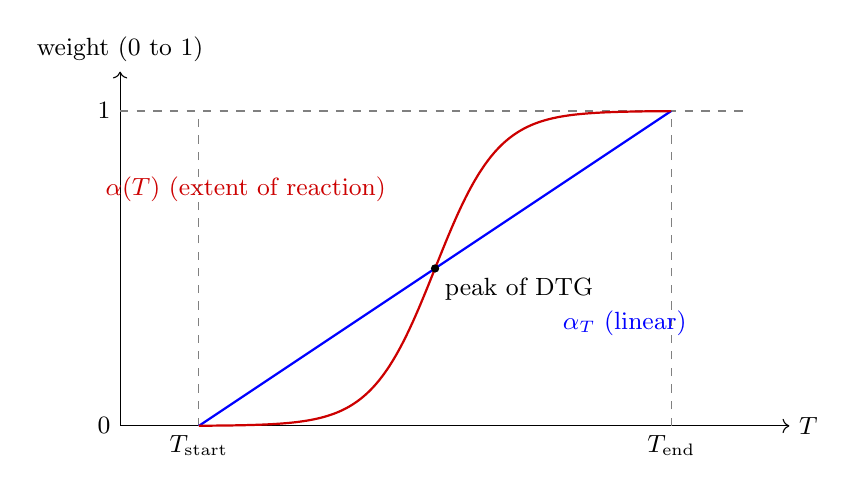
\begin{tikzpicture}[scale=1.0, font=\small]
  \draw[->] (0,0) -- (8.5,0) node[right] {$T$};
  \draw[->] (0,0) -- (0,4.5) node[above] {weight (0 to 1)};
  \node[anchor=east] at (0, 4) {$1$};
  \node[anchor=east] at (0, 0) {$0$};
  \draw[gray, dashed] (0, 4) -- (8, 4);
  \node[anchor=north] at (1, 0) {$T_{\mathrm{start}}$};
  \node[anchor=north] at (7, 0) {$T_{\mathrm{end}}$};
  \draw[gray, dashed] (1, 0) -- (1, 4);
  \draw[gray, dashed] (7, 0) -- (7, 4);
  % Linear: alpha_T (a straight line from (1,0) to (7,4))
  \draw[thick, blue] (1, 0) -- (7, 4);
  \node[blue, anchor=west] at (5.5, 1.3) {$\alpha_T$ (linear)};
  % Sigmoid: alpha(T), sigmoidal between T=1 and T=7 with inflection at T=4
  \draw[thick, red!80!black, smooth, samples=100, domain=1:7]
    plot (\x, {4/(1+exp(-2.5*(\x-4)))});
  \node[red!80!black, anchor=east] at (3.5, 3) {$\alpha(T)$ (extent of reaction)};
  % Mark inflection
  \fill[black] (4, 2) circle (1.5pt) node[anchor=north west] {peak of DTG};
\end{tikzpicture}
\caption{The two weighting functions used in the linear and alpha
baseline modes. Linear ($\alpha_T$) rises uniformly with temperature;
extent-of-reaction ($\alpha(T)$) follows the cumulative mass loss, so
it jumps sharply through the inflection (where the DTG is peaked) and
plateaus on either side. The under-event drift therefore transitions
its slope at different temperatures under the two conventions, which
is why the corresponding integrated mass losses can differ.}
\label{fig:alpha}
\end{figure}

\subsection{An identity worth keeping in mind}

A subtle point: although the constant and linear baselines look quite
different pointwise, they give the \emph{same integrated} mass loss if
you define ``constant'' as the mean of $a_{\mathrm{pre}}$ and
$a_{\mathrm{post}}$. The reason is just calculus --- the integral of a
linear function over an interval equals its midpoint times the width:
\[
  \int_{T_{\mathrm{start}}}^{T_{\mathrm{end}}}
    \bigl[(1-\alpha_T)\,a_{\mathrm{pre}} + \alpha_T\,a_{\mathrm{post}}\bigr]\,
    \mathrm{d}T
  \;=\; \tfrac{1}{2}(a_{\mathrm{pre}} + a_{\mathrm{post}})\,
        (T_{\mathrm{end}} - T_{\mathrm{start}}).
\]
To see this explicitly: substitute $u = (T - T_{\mathrm{start}})/
(T_{\mathrm{end}} - T_{\mathrm{start}})$, so $\alpha_T = u$ and
$\mathrm{d}T = (T_{\mathrm{end}} - T_{\mathrm{start}})\,\mathrm{d}u$.
The integral becomes
$(T_{\mathrm{end}} - T_{\mathrm{start}}) \int_0^1
\bigl[(1-u) a_{\mathrm{pre}} + u\,a_{\mathrm{post}}\bigr]\mathrm{d}u
= (T_{\mathrm{end}} - T_{\mathrm{start}}) \cdot
\tfrac{1}{2}(a_{\mathrm{pre}} + a_{\mathrm{post}})$.
The linear-blend baseline and the mean-slope constant baseline differ
pointwise at every $T$ except the midpoint, and yet their integrals
agree exactly. The pointwise difference cancels by symmetry of the
trapezoid.

For that reason, this package's \code{dtg\_area\_constant} uses
$a_{\mathrm{pre}}$ alone (not the mean), so the constant and linear
columns are genuinely distinct numbers. The alpha column differs from
both only when $a_{\mathrm{pre}}$ and $a_{\mathrm{post}}$ differ
appreciably and the DTG is asymmetric --- which is most of the time
on real data.

\section{When events overlap: deconvolution}

Everything above assumes that each event has quiet baseline on both
sides.  In a hydrated cement paste below \qty{200}{\celsius}, the
calcium-silicate-hydrate, ettringite, and aluminate hydrates dehydrate
on top of each other; there is no quiet region between them. The peak
detector picks up one feature where there are really three or four,
the integration extent sweeps up neighbouring chemistry, and the
reported number is structurally wrong, not just imprecise.

The fix is to model the region as a sum of asymmetric peak shapes and
fit them to the baseline-corrected DTG.

\subsection{The Frazer--Suzuki peak shape}

The standard peak function in thermal-analysis kinetics is the
Frazer--Suzuki form
\[
  y(T; A, T_0, W, b) \;=\;
  A\,\exp\!\left[
    -\frac{\ln 2}{b^{2}}\,
    \ln^{2}\!\left(1 + \frac{2b\,(T - T_0)}{W}\right)
  \right].
\]
Its four parameters have direct interpretations:
\begin{itemize}
  \item $A$ is the peak amplitude (in \unit{\percent\per\celsius}).
  \item $T_0$ is the peak temperature.
  \item $W$ is the full width at half maximum (exactly so in the
        symmetric limit $b \to 0$).
  \item $b$ is an asymmetry. With $b = 0$ the function is a Gaussian.
        Positive $b$ gives a right tail; negative $b$ gives a left
        tail. Real thermal decompositions almost always have left
        tails (a slow ramp-up of reaction rate followed by a sharp
        fall), so fitted values are typically $-0.9 \lesssim b < 0$.
\end{itemize}
The function vanishes outside the temperature range where its log
argument is positive. In mathematical language this property is
called \emph{compact support}: the set of temperatures where the
function is non-zero is bounded (it fits inside a finite interval),
and \emph{outside} that interval the function is exactly zero, not
just very small. This is in contrast to Gaussians and similar bell
shapes, which are technically non-zero everywhere --- they decay
exponentially but never quite reach zero. For deconvolution the
distinction matters in practice: a Frazer--Suzuki peak placed at
$T_0$ contributes exactly zero at temperatures well beyond its own
extent, so a fit on the carbonate region around \qty{700}{\celsius}
cannot be contaminated by the residual exponential tail of a peak the
fit also placed at, say, \qty{200}{\celsius}.  Each peak influences
only the
points within its own bounded range.

\subsection{Fitting a sum of peaks}

If a region $[T_{\mathrm{lo}}, T_{\mathrm{hi}}]$ is believed to contain
$N$ overlapping events, we model the baseline-corrected DTG there as
\[
  y_{\mathrm{model}}(T) \;=\; \sum_{i=1}^{N} y(T; A_i, T_{0,i}, W_i, b_i)
\]
and fit the $4N$ parameters by nonlinear least squares
(\code{scipy.optimize.curve\_fit}). Initial guesses for $T_{0,i}$ come
from a peak detector on $y_{\mathrm{model}}$ itself; widths default
to a fraction of the region width; asymmetries start at zero. Bounds
keep $A \ge 0$, $W \ge \qty{1}{\celsius}$, and $|b| \le 0.95$ to avoid
degenerate fits.

The mass loss attributed to peak $i$ is its integral, computed
numerically on the same $T$ grid. The peak integrals sum to the total
integrated mass loss for the region under the chosen baseline.

\subsection{The region must extend into quiescent baseline flanks}

By far the most common deconvolution mistake is choosing a region that
starts or ends inside the tail of a real event.  We use the term
\emph{quiescent baseline flank} for the interval of temperature on
either side of the fitted region in which the mass signal is dominated
by slow, near-linear drift and no active decomposition; this is the
substrate on which a defensible pre- or post-event baseline can be
fitted.  The package fits the pre-baseline to a
\qty{20}{\celsius}-wide window just below $T_{\mathrm{lo}}$ and the
post-baseline to a \qty{20}{\celsius}-wide window just above
$T_{\mathrm{hi}}$.  If either of those windows is contaminated by
ongoing chemistry --- i.e., if it does not lie in a quiescent flank
--- the baseline slope is wrong, the corrected DTG is wrong, and the
deconvolved per-peak masses are nonsense, even though the fit
converged.

A worked example.  On a clean calcite (theoretical mass loss
\qty{43.97}{\percent}), a deconvolution with
$T_{\mathrm{lo}} = \qty{700}{\celsius}$, which sits well inside the
rising edge of the decarbonation event, gives per-peak mass losses of
approximately \qtylist{21;27;27}{\percent} under the three baseline
modes.  Widening to $T_{\mathrm{lo}} = \qty{540}{\celsius}$ --- which
puts the leading window into a genuinely quiescent flank --- gives
\qtylist{43.6;43.7;43.7}{\percent}: a \qty{0.3}{\percent} spread,
agreeing with theory.  The fit converged in both cases.  The only
difference is whether the leading window saw chemistry or not.

\section{What deconvolution cannot do}

It is important to be honest about the resolution limit of any
single-ramp TGA experiment. Deconvolution is not magic: it imposes a
parameterized peak shape on the data and finds the best-fit
parameters, but it cannot extract information that is not in the
trace.

Two events that overlap sufficiently --- such that no shoulder or
inflection is visible in the DTG --- are \emph{mathematically
unresolvable} from one ramp. Many different decompositions of the
total signal into two peaks fit equally well; the parameters trade
off against one another, and the result depends mostly on the initial
guess. The fit reports tiny residuals and nonsense uncertainties; if
you re-ramp the same sample at a different heating rate, you get a
different ``deconvolution'' that fits equally well.

Honest options when this happens are:

\begin{itemize}
  \item \emph{Multi-rate (isoconversional) experiments.} Ramp the same
        sample at, e.g., \qtylist{5;10;20;40}{\kelvin\per\minute},
        and analyse the apparent activation energy as a function of
        $\alpha$. Events with different kinetic signatures separate
        in the multi-rate data even if they overlap at any single
        rate. This is the approach the ICTAC kinetics committee
        recommends.
  \item \emph{Coupled techniques.} TGA--MS (mass spectrometer on the
        evolved gas) or TGA--FTIR identifies \emph{what} is being
        released, so you can attribute mass to chemistry directly
        rather than guessing from the temperature alone.
  \item \emph{Sample preparation.} Sometimes the right answer is not
        better analysis but a different experiment --- e.g., washing
        away the carbonate phase before the ramp to isolate the
        portlandite peak.
\end{itemize}

The package will happily deconvolve any region you give it, with any
number of peaks you ask for. It is your job to confirm that the data
actually contain shoulders that justify the number of peaks --- the
diagnostic PNG is your friend here. If the corrected DTG in the region
is genuinely a single asymmetric bump, fitting two Frazer--Suzuki
peaks to it will give you two peaks with arbitrary parameter values
that sum to the right shape but mean nothing individually.

\section{A practical caveat: $\mathrm{CaCO}_3$ polymorphs}

If your samples are $\mathrm{CaCO}_3$ powders or contain
$\mathrm{CaCO}_3$ phases, a chemistry caveat worth knowing: the three
common $\mathrm{CaCO}_3$ polymorphs --- aragonite, vaterite, and
calcite --- do \emph{not} have distinguishable thermal decomposition
signatures in TGA. Both aragonite and vaterite undergo a solid-state
polymorphic transformation to calcite well before
$\mathrm{CaCO}_3 \to \mathrm{CaO} + \mathrm{CO}_2$:

\begin{itemize}
  \item Vaterite $\to$ calcite, roughly \qtyrange{320}{460}{\celsius}.
  \item Aragonite $\to$ calcite, roughly \qtyrange{380}{490}{\celsius}.
  \item $\mathrm{CaCO}_3 \to \mathrm{CaO} + \mathrm{CO}_2$ (calcite),
        roughly \qtyrange{600}{800}{\celsius}, depending on crystallinity,
        partial pressure of $\mathrm{CO}_2$, and heating rate.
\end{itemize}

Whatever polymorph you put in the pan, by the time decarbonation
happens the sample is calcite. The decarbonation DTG cannot, in
principle, distinguish ``calcite that has always been calcite'' from
``aragonite that became calcite at \qty{430}{\celsius}.''  Coupled techniques
--- room-temperature XRD, FT-Raman, or FTIR --- are required for
polymorph identification. This has been documented since
Passe-Coutrin \emph{et al.} (1992) and is the explicit subject of
Kontoyannis \& Vagenas (\emph{Analyst} \textbf{125}, 251, 2000), the
standard reference.

The polymorph transformations themselves \emph{are} visible in DSC
(they are weakly exothermic), and they show up as small features in
DTG if the polymorphic transition is accompanied by water release
from a hydrate carbonate, but the \qty{700}{\celsius} decarbonation peak by
itself is silent on which polymorph you started with.

\section{Method agreement as a diagnostic}

Putting all of this together, the workflow the package supports is:

\begin{enumerate}
  \item Run the detection and the five mass-loss columns.
  \item For each event, look at the three DTG-area columns
        ($\code{constant}$, $\code{linear}$, $\code{alpha}$). If they
        agree to within a couple of percent and lie close to
        $\code{tangent}$, the answer is trustworthy --- the event is
        cleanly isolated and any of the methods would do.
  \item If the three DTG-area values \emph{disagree}, or if any of
        them differs greatly from $\code{tangent}$, treat the number
        as suspect. The event extent is being polluted by overlapping
        chemistry, and no baseline choice can fix it; the integration
        limits themselves are wrong.
  \item In that case, run a deconvolution over a region wide enough
        to include the event \emph{and} \qty{20}{\celsius} of
        quiescent baseline flank on each side, with $N$ peaks chosen
        to match what the DTG plot suggests.
  \item Confirm that the per-peak masses agree across the three
        baseline modes. If they do, those numbers are trustworthy. If
        they still disagree, widen the region or reconsider $N$.
\end{enumerate}

The point is that the package is not telling you what the answer is.
It is telling you when you can trust the answer it computed, and when
you need to do more work. The agreement (or disagreement) of three
methods that ought to give the same answer under good conditions is
itself the validation signal --- a useful guard against an over-confident
single number from a single method.

\section*{Further reading}

\begin{itemize}[leftmargin=*, label={}]
  \item Savitzky, A.; Golay, M. J. E. (1964). ``Smoothing and
        Differentiation of Data by Simplified Least Squares
        Procedures.'' \emph{Anal. Chem.} \textbf{36}, 1627--1639.
  \item Vyazovkin, S.; \emph{et al.} (2011). ICTAC Kinetics Committee
        recommendations for performing kinetic computations on thermal
        analysis data. \emph{Thermochim.\ Acta} \textbf{520}, 1--19.
  \item Vyazovkin, S.; \emph{et al.} (2020). ICTAC Kinetics Committee
        recommendations for analysis of multi-step kinetics.
        \emph{Thermochim.\ Acta} \textbf{689}, 178597.
  \item Gibson, R.; Simmons, M.~J.~H.; Stitt, E.~H.; Horsburgh, L.;
        Gallen, R.~W. (2022). ``Selection of Formal Baseline
        Correction Methods in Thermal Analysis.''
        \emph{Chem.\ Eng.\ Technol.} \textbf{45}(2), 238--248.
  \item Kontoyannis, C.~G.; Vagenas, N.~V. (2000). ``Calcium Carbonate
        Phase Analysis Using XRD and FT-Raman Spectroscopy.''
        \emph{Analyst} \textbf{125}, 251--255.
  \item Lothenbach, B.; Durdzi\'nski, P.; De Weerdt, K. (2017).
        Thermogravimetric analysis, in \emph{A Practical Guide to
        Microstructural Analysis of Cementitious Materials},
        Scrivener, K., Snellings, R., Lothenbach, B., eds., CRC Press.
\end{itemize}

\end{document}
